
\section{Experimental Setup}\label{results:setup}

An experiment consists of a set of resource-exchange graph instances executed
with a collection of configured solvers. When a solution is found, the solution
(i.e., the flow vector), the time required to reach the solution, and the
objective value (i.e., the dot-product of cost and flow vectors) are
recorded. Because solution time is a quantity of interest, all instances in an
experiment must be executed on homogeneous architecture. Furthermore, all
experiments must be executed on equivalent, homogeneous architecture in order to
quantify valid comparisons in solutions times across experimental campaigns.

Six execution nodes on UW-Madison Advanced Computing Initiative (ACI) HTCondor
system form the homogeneous environment used to conduct the experiments herein
described. Each execute node is comprised of an 2.90 GHz eight-core,
sixteen-thread, Intel Xeon E5-2690 \cite{intelproc} processor with 128 GB of
RAM. Processor hyper-threading was disabled for the duration of the experimental
campaign to allow comparisons between solution times.

For each experimental study, an input database consisting of persisted resource
exchange graph instances is generated. A copy of the database is transferred
from a user's submit node to each of the six execution nodes. A WorkQueue master
process is initiated. Sixteen workers per node are initialized using WorkQueue's
\texttt{condor\_submit\_workers} CLI. The master maintains a queue of instances
to be solved, assigning instances to workers as workers become available. Upon
completion, the input database is removed from each execution node, and the
results are collected from the user's submit node. The resulting database is
then post-processed and analyzed.

\subsection{Solvers and Formulations}

Three solvers are executed for each resource exchange graph instance: the Greedy
Heuristic, described in \S \ref{abm:dre:nfctp:heur}, COIN's LP solver
(COIN-CLP), and COIN's branch-and-cut solver (COIN-CBC). Each problem instance
is constructed as a \texttt{ExchangeGraph}, i.e., at the \textit{exchange layer}
shown in Figure \ref{fig:dre_impl} and Figure \ref{fig:dre_time}. The Greedy
Heuristic is applied directly to the \texttt{ExchangeGraph}. The CLP and CBC
solvers require a translation to the \textit{formulation layer}. The CLP solver
is applied to the LP formulation of the NFCTP and the CBC solver is applied to
the MILP formulation. The solution time, $t_s$ of a given solver is defined as
the time required to return a vector of arc flows given an
\texttt{ExchangeGraph} instance as shown in Figure \ref{fig:dre_time}.

\begin{equation}\label{eqn:solnt}
t_s = t_f - t_i
\end{equation}

\begin{figure}
  \begin{center}
    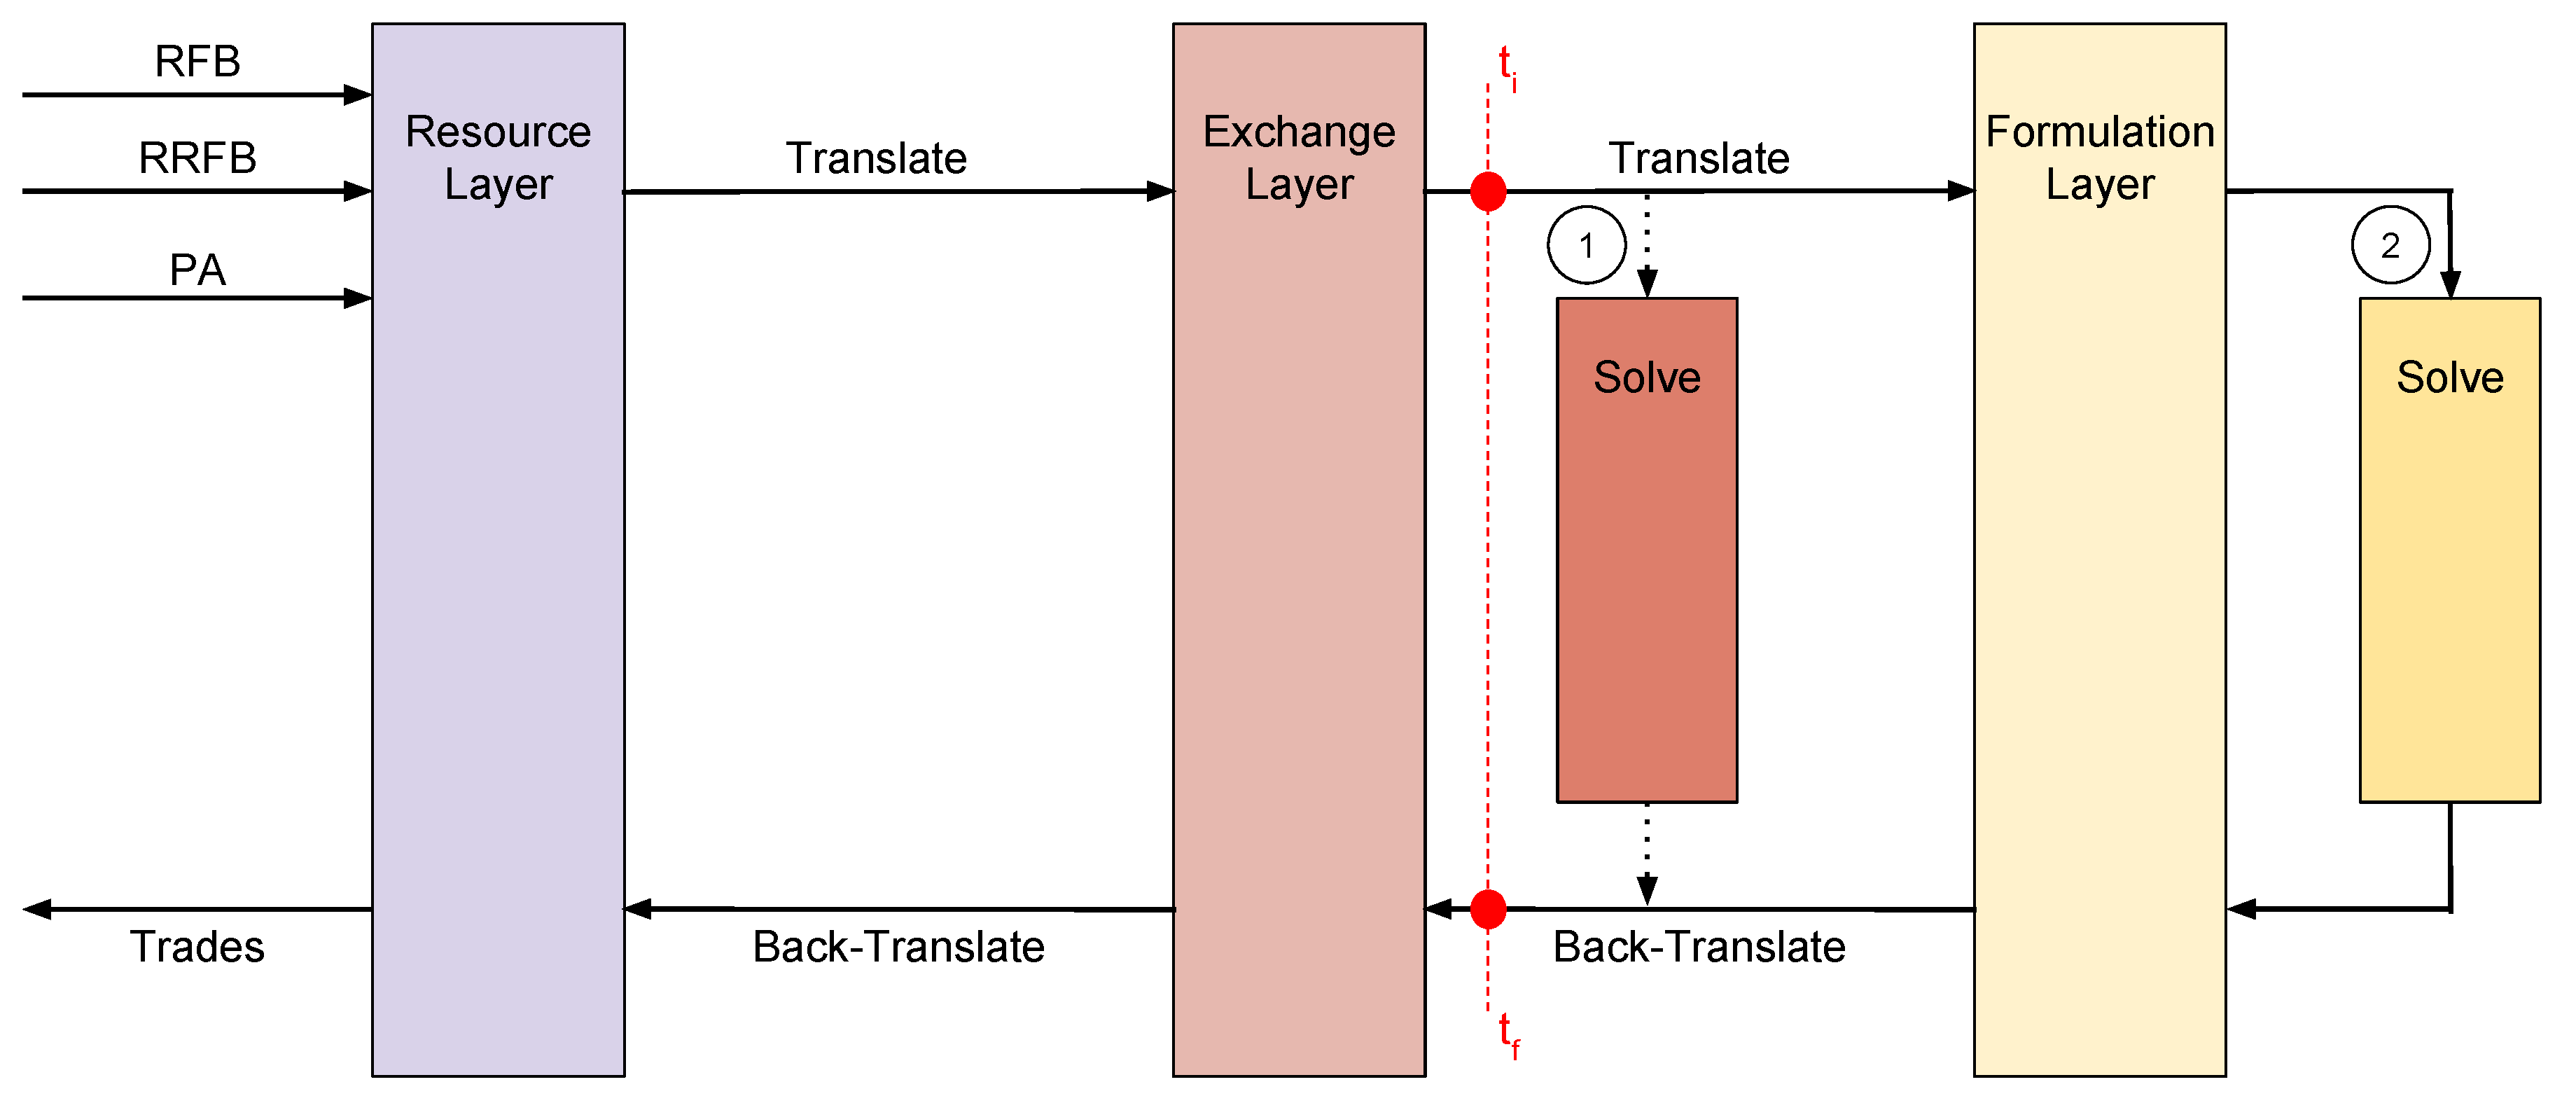
\includegraphics[width=\textwidth]{exchange_xlation_timing.pdf}
    \caption{
      \label{fig:dre_time}
      The time points for comparing different solutions using Equation \ref{eqn:solnt}.}
  \end{center}
\end{figure}

The Greedy Heuristic has $\mathcal{O}(N_A)$ scaling, where $N_A$ is the number
of arcs in the system. In the worst case, i.e., in highly constrained systems,
every arc will be processed. As both CLP and CBC solve NP-Hard problems, there
is no \textit{a priori} expected performance behavior.

\subsection{Parameter Variation}

\S \ref{method:setup:params} describes the parameters defining both Front and
Back-End exchanges. Each combination of fundamental parameters represents a
significant modeling assumption. Therefore, every experiment is conducted for
every combination of fundamental parameters, comprising eighteen combinations in
total. For exchange type, a reference instance parameter vector is
chosen. Experiments, then, are conducted by using either the reference vector or
perturbing instance parameter values from the reference vector and comparing
output.

Reference instance parameter vectors for front and back-end exchanges are shown
in Tables \ref{tbl:front_ref_params} and \ref{tbl:back_ref_params},
respectively. Reactor population and core composition values were chosen in line
with what a user might reasonably find in a simulation, such as a 75\%-25\%
thermal-to-fast reactor split and 33\% possible MOX-fuel residency in thermal
reactors. Support facility population values were chosen to model a ``worst
case'' simulation. The notion of a ``worst case'' simulation is defined as one
in which supporting facilities' services do not fully meet the demand of the
reactor population. Therefore, the resulting exchanges are highly constrained,
resulting in ``worst case'' behavior for the Greedy Heuristic. 

\begin{table}[h!]
\centering
\caption{Reference Values for Front-End Exchange Instance Parameters.}
\label{tbl:front_ref_params}
\begin{tabular}{|c|c|}
\hline
Parameter    & Reference Value
\\ \hline
$r_{rx, \text{Th}}$   & 0.75 
\\ \hline
$r_{rx, \text{FThOX}}$ & 0.25
\\ \hline
$r_{l, c}$ & 1
\\ \hline
$f_{mox}$     & 0.33
\\ \hline
$r_{s, \text{Th}}$ & 0.08
\\ \hline
$r_{s, \text{TMOX}, \text{UOX}}$ & 1.
\\ \hline
$r_{s, \text{FMOX}}$ & 0.2
\\ \hline
$r_{s, \text{FThOX}}$ & 0.2
\\ \hline
$r_{inv, proc}$   & 1
\\ \hline
\end{tabular}
\end{table}

\begin{table}[h!]
\centering
\caption{Reference Values for Back-End Exchange Instance Parameters.}
\label{tbl:back_ref_params}
\begin{tabular}{|c|c|}
\hline
Parameter    & Reference Value
\\ \hline
$r_{rx, \text{Th}}$   & 0.75 
\\ \hline
$r_{rx, \text{FThOX}}$ & 0.25
\\ \hline
$r_{l, c}$ & 1
\\ \hline
$f_{mox}$     & 0.33
\\ \hline
$r_{s, \text{Th}}$ & 0.08
\\ \hline
$r_{s, \text{TMOX}, \text{UOX}}$ & 1.
\\ \hline
$r_{s, \text{FMOX}}$ & 0.2
\\ \hline
$r_{s, \text{FThOX}}$ & 0.2
\\ \hline
$r_{s, \text{Repo}}$   & 0.2
\\ \hline
$d_{\text{Th}}$   & {UOX: 2/3, TMOX: 1/3, FMOX: 0}
\\ \hline
$d_{\text{FMOX}}$   & {UOX: 1/4, TMOX: 0, FMOX: 3/4, FThOX: 0}
\\ \hline
$d_{\text{FThOX}}$   & {UOX: 1/4, TMOX: 0, FMOX: 0, FThOX: 3/4}
\\ \hline
\end{tabular}
\end{table}

\subsection{Analysis Metrics}

The most obvious metrics to compare between solutions is the solution time,
$t_s$, and objective function value $z$,

\begin{equation}\label{eqn:obj_flow}
z = \sum_{(i, j) \in A} c_{i, j} x_{i, j}.
\end{equation}

For any given instance, the optimal objective value, $z^*$, is associated with a
set of flows, $x^*$. By definition, an optimal solution will have a lower or
equivalent system cost than any feasible solution.

While the objective function is minimized in the NFCTP formulations, it
necessarily includes flow along false arcs. Considering all arcs that exist both
in the formulation and the simulation, $A_{\text{sim}}$, another valid
comparison is dot product of preference and flow vectors. This value can be
considered the ``simulation objective'', i.e.,

\begin{equation}\label{eqn:sim_flow}
z_{\text{sim}} = \sum_{(i, j) \in A_{\text{sim}}} p_{i, j} x_{i, j}.
\end{equation}

A similar guarantee cannot be provided for $z^*_{\text{sim}}$. That is, while
$z^* \leq z$ is true in cost space, $z^*_{\text{sim}} \geq z_{\text{sim}}$ is
\textit{not} necessarily true.

%% The preference vector, $\vec{p}$, can be divided into its two components,
%% $\vec{p} = \vec{p}_c + \vec{p}_l$. If $f_{\text{loc}}$ is zero, then, by
%% definition, $\vec{p}_l = 0$, otherwise, it is comprised of non-zero
%% components. $\vec{p}_c$, however, is invariant under all values of
%% $f_{\text{loc}}$. Therefore, the commodity contribution of the simulation
%% objective, shown in Equation \ref{eqn:cpref_flow} is also an interesting
%% metric. It allows for direct investigation of the effect of adding
%% location-based preferences to the system. Furthermore, comparisons can be made
%% between systems with coarse and fine location-based preferences using this
%% metric.

%% \begin{equation}\label{eqn:cpref_flow}
%% z^c_{\text{sim}} = \sum_{(i, j) \in A_{\text{sim}}} p^c_{i, j} x_{i, j}.
%% \end{equation}

Each of the above metrics compare aggregate values between solutions. That is,
comparisons are being made at a macroscopic scope. For any two solutions to
identical problem instances, though, more detailed comparisons can be made. The
individual flow values, and values derived therefrom, can be compared directly
using a well-known normative measure. One example is the root mean square (RMS)
of constituents of the objective function, shown in Equation
\ref{eqn:rms_flow}.

\begin{equation}\label{eqn:rms_flow}
RMS_{\text{z}} = \sqrt{ \frac{1}{N} \sum_i c_i^2 (x_{i, 1} - x_{i, 2}) ^2 }
\end{equation}

While such an analysis is common in the realm of nuclear engineering, it is less
appropriate for comparing solutions to optimization problems. An instance of an
optimization problem may be \textit{degenerate}, i.e., it may have multiple
equivalent optimal solutions. Consider a two-arc system with arc costs of unity
and a total flow constraint of unity. A spectrum equivalent solutions exist
between $(0, 1)$ and $(1, 0)$. When comparing any solution, the difference in
objective function value is, necessarily, zero. However, using an RMS analysis,
the solutions of $(0, 1)$ and $(1, 0)$ would report the largest possible
error. Therefore, only metrics that involve aggregate measures of solutions are
used in the following analysis.
